\documentclass{beamer}
\usepackage[utf8]{inputenc}
\usepackage{macro}
\usepackage{wrapfig}
\usepackage{graphicx}

\title{Deep RL from Human Preferences}

\begin{document}
\frame{\titlepage}

\begin{frame}{Problem}
  Designing reward function for complex RL system is hard
\end{frame}

\begin{frame}{Approaches}
  \begin{itemize}
    \item \textbf{Learn it} Learn what is good behavior vs bad behavior through supervised learning
    \item \textbf{Inverse RL} Given trajectories from an optimal policy, infer a reward function that results 
      the optimal policy. 
      \href{https://ai.stanford.edu/~ang/papers/icml00-irl.pdf}{Ng, Russell 2000}
    \begin{itemize}
      \item many reward functions can result in the same optimal policy
    \end{itemize}
  \end{itemize}

  The paper explores approach 1.
\end{frame}

\begin{frame}{Overview of the methods}
  \begin{itemize}
    \item collect RL agent's behavior
    \item send video clips of those behavior to human labelers
    \item human labelers see two behaviors at once, they provide feedbacks
      on which one of them is better
    \item train a reward predictor to fit human preference
    \item continue training the RL agent to please the reward predictor
  \end{itemize}

\begin{wrapfigure}{r}{0.5\textwidth}
%\vspace{-10mm}
\begin{center}
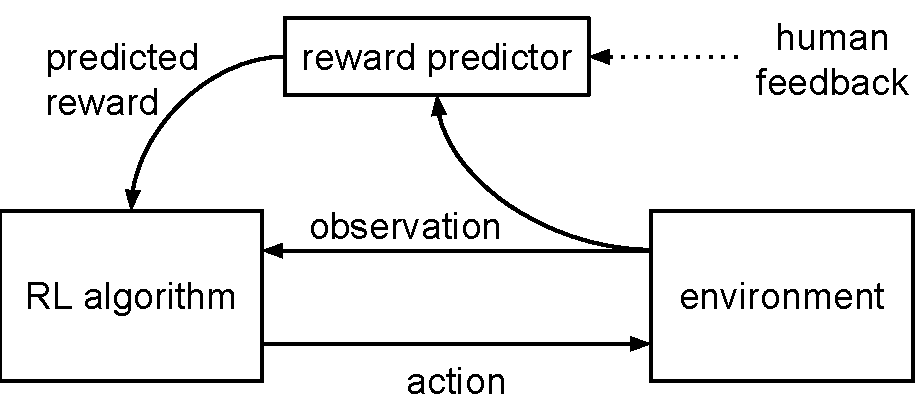
\includegraphics[width=0.45\textwidth]{setup.pdf}
\end{center}
\caption{Schematic illustration of our approach:
the reward predictor is trained asynchronously from comparisons of trajectory segments,
and the agent maximizes predicted reward.}
\label{fig:reward-feedback-schema}
\end{wrapfigure}

See section 2 of the paper for more details
\end{frame}

\begin{frame}{Problems with the methods}
\begin{itemize}
  \item cost of labels
  \item reward predictor might return a wrong scale
  \item when the RL policy is near random, comparison tasks
    for human labelers are not meaningful
\end{itemize}
\end{frame}

\begin{frame}{Design space}
\begin{itemize}
  \item Single reward predictor or an ensemble of reward predictors?
    They choose ensemble as baseline.
  \item When to query for human feedbacks?
    They use variance among predictors as a heuristic measure of 
    information gain. 
  \item how long the video segments to show to human lablers. 
    They used vidoe segmentas lasted from 3 - 5 seconds.
\end{itemize}
See Ablation Studies in 3.3 for a complete list of design choices. 
\end{frame}

\begin{frame}{Experiment results}
Experiements performed on MuJoCo and Atari. They compared RL agent's 
performance when trained with 
  \begin{itemize}
    \item traditional reward
    \item synthetic feedbacks from an oracle. The oracle has access to 
      true reward, and provide feedbacks based on the true reward
    \item human feedbacks
  \end{itemize}

High level observations:
\begin{itemize}
  \item real reward does not result the best performance in many cases
  \item human feedback on Ant resulted much faster learning
\end{itemize}

See section 3 for more details
\end{frame}

\begin{frame}{Experiment results (continued)}
Learning novel behaviors. See section 3.2
\end{frame}

\begin{frame}{Experiment results (continued)}
Why human feedbacks are especially useful for Ant?

  \href{https://www.youtube.com/results?search_query=ant+mujoco}{Link to demo}

Reward:
\[
    r_t = x_t - 0.5 \times ||a_t||^2_2 - 0.0005 \times ||s_t||^2_2 + 1
\]

\href{http://proceedings.mlr.press/v139/furuta21a/furuta21a-supp.pdf}{Link to MuJoCo env reward}
\end{frame}

\begin{frame}{Experiment results (continued)}
Why Qbert has such a bad performance when trained with human feedbacks

  \href{https://www.youtube.com/watch?v=vkZhWsiHCqM&t=141s}{Link to Demo}

My guess: 3-5 vidoe clips is not sufficient for human lablers to 
figure out what is a good behavior.
\end{frame}

\begin{frame}{Ablation Studies}
See section 3.3 for details. 
\begin{itemize}
  \item impactful factors: length of segment, ensemble
  \item counter-intuitive observations: uncertainty based query strategy
        does not seem to outperform random queries
\end{itemize}
\end{frame}


\end{document}
